% basic nastaveni
\documentclass[12pt]{article}
\setlength{\parindent}{0pt}
\setlength{\parskip}{1em}
\usepackage[utf8]{inputenc}
\usepackage[czech]{babel}
\usepackage[T1]{fontenc}
\usepackage{graphics}
\usepackage{caption}
\usepackage{hyperref}
\usepackage{xcolor}
\usepackage{float}

% matematicke package
\usepackage{amsmath}
\usepackage{amsfonts}
\usepackage{amssymb}
\usepackage{geometry}
\geometry{margin=2.5cm}
\usepackage{pgfplots}
\pgfplotsset{compat=1.18}
\usepackage{mathrsfs}

\title{Maturitní otázka číslo 6: Nealgebraické funkce}
\author{}
\date{}

\begin{document}
\maketitle
\subsection*{Exponenciální funkce}
Exponenciální funkce $f$ má tvar $f(x) = a^x, a \in \mathbb{R}, a > 0, a \ne 1$. Funkce je na celém
definičním oboru konvexní a prostá. Funkce je omezená zdola číslem $0$, obor hodnot je $(0, \infty)$
a definční obor jsou všechna reálná čísla. Vlastnosti i graf se zásadně mění od toho, zda je $a$ větší
nebo menší než jedna. Pokud je $a$ v intervalu od $(0, 1)$, funkce je klesající. Pokud je $a$ v
intervalu od $(1, \infty)$, je rostoucí.

\begin{figure}[H]
    \centering
    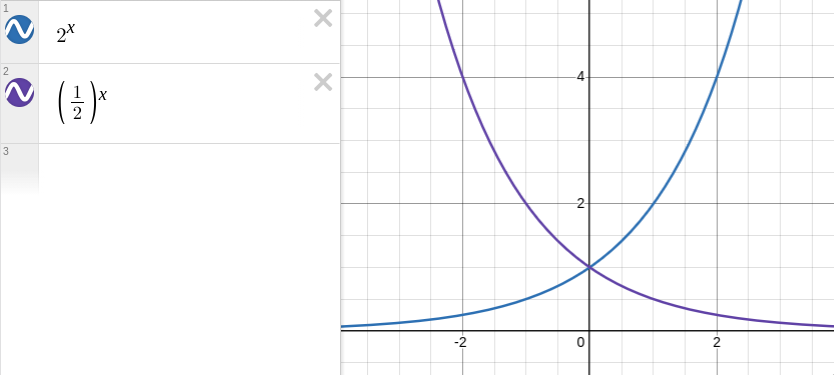
\includegraphics[width=0.6\textwidth]{pictures/exponencilani_funkce.png}
    \caption*{}
\end{figure}

\subsection*{Logaritmické funkce}
Logaritmická funkce má předpis $y = \log_{a} x, a \in \mathbb{R}, a > 0, a \ne 1$. Tento zápis čteme
jako logaritmus čísla $x$ o základu $a$. Číslo $a$ se nazývá základ nebo báze a číslo $x$
je argument. Logaritmická funkce je inverzní k exponenciální, tedy platí $y = \log_a x \Leftrightarrow
a^y = x$. Existují dva speciální logaritmy. Prvním z nich je přirozený, který se značí jako $\ln x$.
Ten má jako bázi Eulerovo číslo $e$. Druhým z nich je logaritmus s bází $10$, který se zapisuje
jako $\log x$. Definiční obor je $D(f) = (0, \infty)$ a obor hodnot je $H(f) = \mathbb{R}$.
Vlastnosti funkce jsou rozdílné pro $a > 1$ a $0 < a < 1$. Pokud je $a > 1$, funkce je rostoucí
a konkávní. Pokud je $0 < a < 1$, funkce je klesající a konvexní.

\begin{figure}[H]
    \centering
    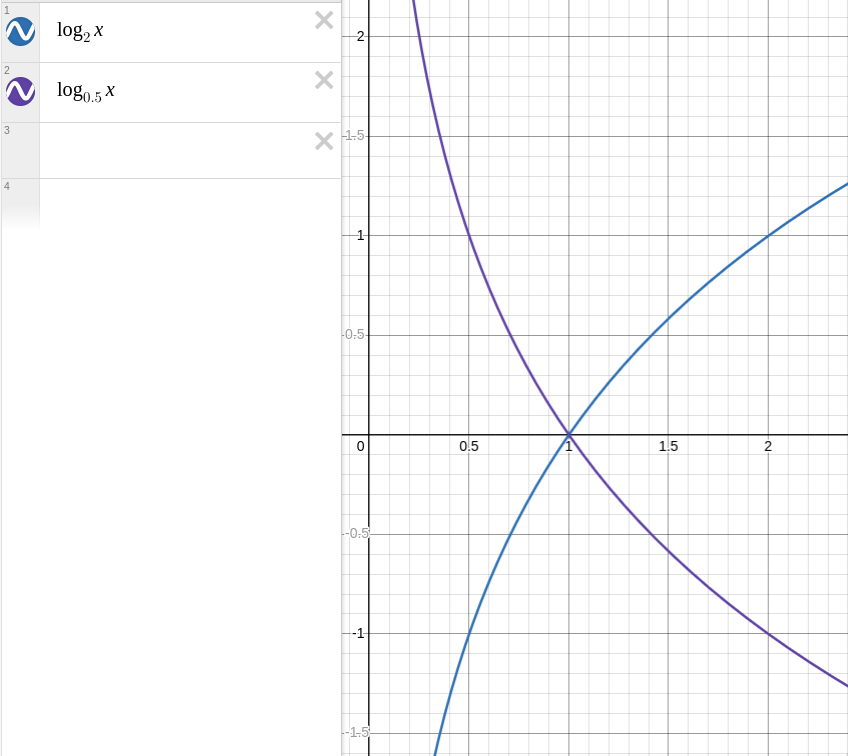
\includegraphics[width=0.6\textwidth]{pictures/logaritmicke_funkce.png}
    \caption*{}
\end{figure}
\subsection*{Operace s mocninami a logaritmy}

Násobení mocnin: $a^n \cdot a^m = a^{n+m}$

Dělení mocnin: $\frac{a^n}{a^m} = a^{n-m}$

Umocňování mocniny: $(a^n)^m = a^{n \cdot m}$

Převracení záporné mocniny: $a^{-n} = \frac{1}{a^n}$

Logaritmus součinu: $\log_a(x \cdot y) = \log_ax + \log_ay$

Logaritmus podílu: $\log_a (\frac{x}{y}) = \log_ax - \log_ay$

Logaritmus mocniny: $\log_a(x^k) = k \cdot \log_ax$

Změna základu: $\log_ax = \frac{\log_bx}{\log_ba}$

Přepis čísla na jiný základ: $x = a^{\log_ax}$
\end{document}
